\documentclass[journal]{IEEEtran}

\usepackage{csquotes}


\usepackage{cite}


% *** GRAPHICS RELATED PACKAGES ***
%
\ifCLASSINFOpdf
  \usepackage[pdftex]{graphicx}
  % declare the path(s) where your graphic files are
  \graphicspath{{./pdf/}{./jpeg/}}
  % and their extensions so you won't have to specify these with
  % every instance of \includegraphics
  \DeclareGraphicsExtensions{.pdf,.jpeg,.png}
\else
  % or other class option (dvipsone, dvipdf, if not using dvips). graphicx
  % will default to the driver specified in the system graphics.cfg if no
  % driver is specified.
  \usepackage[dvips]{graphicx}
  % declare the path(s) where your graphic files are
  \graphicspath{{./eps/}}
  % and their extensions so you won't have to specify these with
  % every instance of \includegraphics
  \DeclareGraphicsExtensions{.eps}
\fi

\usepackage{array}
\usepackage{url}

\hyphenation{op-tical net-works semi-conduc-tor}

\begin{document}

\title{Revealing Middleboxes Interference}

\author{Raphael~Javaux, University of Liege}

% The paper headers
\markboth{Network Measurement and Monitoring, April~2014}
         {Revealing Middleboxes Interference}
% The only time the second header will appear is for the odd numbered pages
% after the title page when using the twoside option.

\maketitle

% \begin{IEEEkeywords}
% IEEEtran, journal, \LaTeX, paper, template.
% \end{IEEEkeywords}

\section{Introduction}

\IEEEPARstart{I}{} wrote a Python utiliy to collect some statistics using enhanced traceroutes. These traces have been used to compute the average path lengths over the Internet, the fraction of routers supporting the RFC1812 or the presence of a TCP proxy.

\subsection{Sample set}

Samples traceroutes were collected over the set of the 5,000 most popular websites from Alexa. Traceroutes were performed by sending TCP SYN segments on port 80 with a TTL ranging from 1 to 30. Responses were collected within a timeout of 2 seconds.

\subsection{Vantage points}

Two vantage points were used to collect data. The first was a personal Internet connection from the local cable operator (\textit{VOO}) whereas the second one was a fast symetric link to a dedicated server in France (\textit{OVH}). VOO was located behind a NAT while OVH was not. Both VPs were using the same input set of websites.

\subsection{Scripts}

Scripts used to collect statistics are located in the \textit{scripts} sub-directory of this assignment. The \textit{main.py} Python 2.7 script was used to probe the top websites whereas \textit{proxy.py} was used to test the presence of a TCP proxy in front of a website. \\
Both scripts accept a set of command line arguments. The \textit{--help} parameter will list, for each script, the set of allowed command line arguments. The \textit{README} file contains some command examples. \\
Running \textit{main.py} over 5,000 websites takes a few hours.

\section{Q1: Path statistics}

Table \ref{tab:general_stats} shows the general statistics about the collected data. On both vantage points, almost every website were reachable. Unreachable websites were wether too far two fall in the TTL range (mostly Asian hosts) or unresolveable domains (i.e. the \textit{akamaihd.net} domain is provided by Alexa but could not be used directly to reach HTTP content as it does not resolve to any host). As it could be expected, the average number of hops is lower from the dedicated server as compared to the personal broadband connection. \\
Table \ref{tab:router_stats} shows detailed router statistics. Un-silent routers are routers which responded to expired TTLs with a \textit{time-expired} ICMP packet. The higher proportion of un-silent routers in the VOO vantage point is probably caused by the higher number of ISP-level un-silent routers to systematically cross for every website. Unique un-silent is the number of different routers which responded to expired TTLs. \\
Table \ref{tab:private_routers} shows the proportion of routers responding to expired TTLs which anounce private IPs. The number of private routers in the VOO vantage point is higher as the two first routers were announcing private IPs. When comparing the number of different routers announcung private IPs, both vantage points exposed a very low fraction of private routers. \\
Figure \ref{fig:cdf} shows in blue the CDF of destination distances from both vantage points. Paths are significantly smaller on the OVH vantage point. There is almost no website at less than 4 hops for both vantage points.

\begin{table}[h]
    \begin{center}
        \begin{tabular}{ | c | c | c | }
            \hline
            VP   & Reachable sites & AVG path hops \\ \hline
            VOO  & 4807 (96.1\%)   & 14.9          \\ \hline
            OVH  & 4805 (96.1\%)   & 12.7          \\
            \hline
        \end{tabular}
    \end{center}
    \caption{General statistics on the collected data.}
    \label{tab:general_stats}
\end{table}

\begin{table}[h]
    \begin{center}
        \begin{tabular}{ | c | c | c | c | }
            \hline
            VP   & Routers & Un-silent      & Unique un-silent   \\ \hline
            VOO  & 71462   & 62378 (87.3\%) & 9429               \\ \hline
            OVH  & 60896   & 46011 (75.6\%) & 9749               \\
            \hline
        \end{tabular}
    \end{center}
    \caption{General statistics on routers.}
    \label{tab:router_stats}
\end{table}

\begin{table}[h]
    \begin{center}
        \begin{tabular}{ | c | c | c | c | }
            \hline
            VP   & Priv. un-silent & Unique priv. un-silent \\ \hline
            VOO  & 9580 (15.4\%)             & 6 (0.06\%)   \\ \hline
            OVH  & 102 (0.2\%)               & 47 (0.5\%)   \\
            \hline
        \end{tabular}
    \end{center}
    \caption{Un-silent routers announcing private IPs.}
    \label{tab:private_routers}
\end{table}

\begin{figure}[!t]
    \centering
    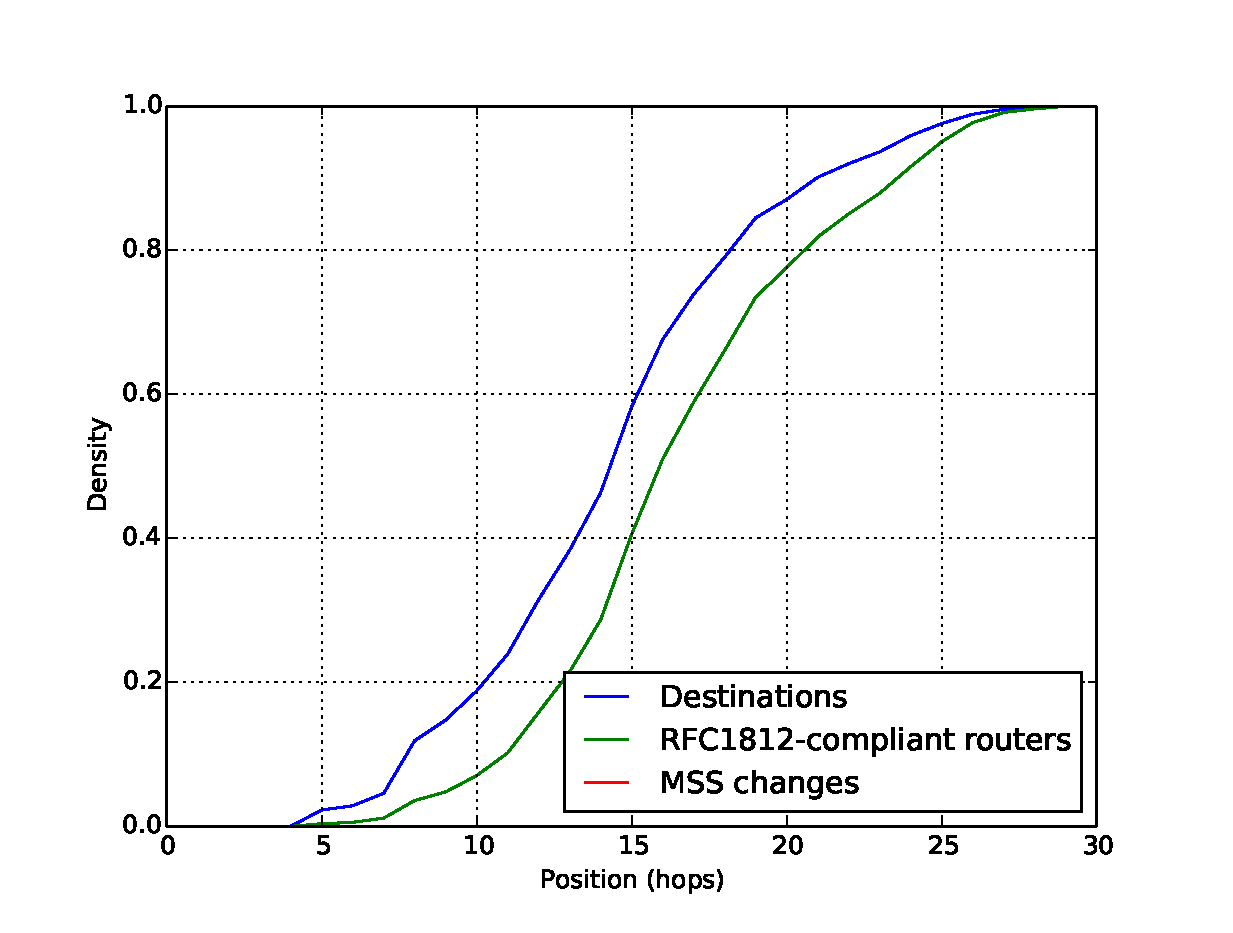
\includegraphics[width=3.5in]{cdf_voo}
    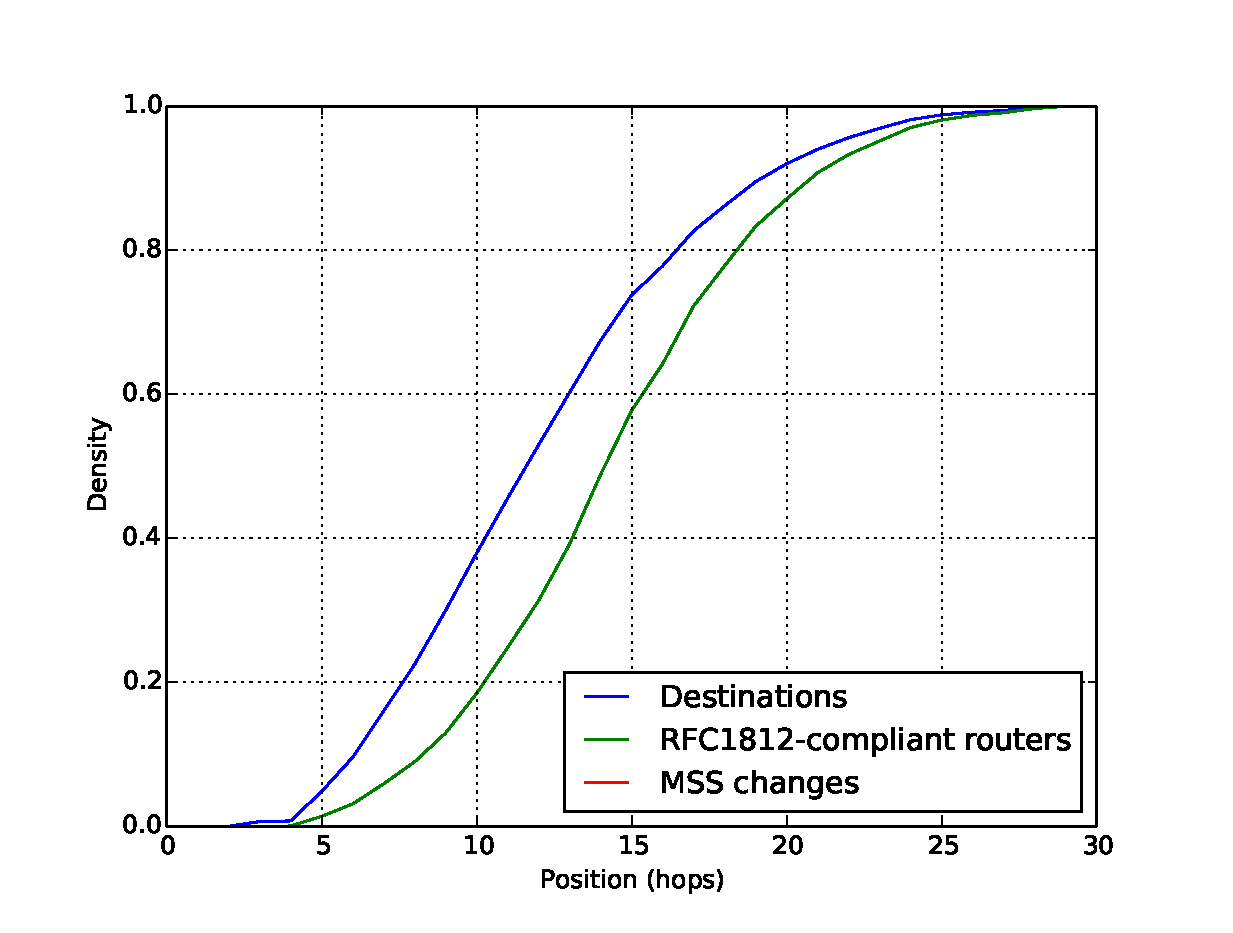
\includegraphics[width=3.5in]{cdf_ovh}
    \caption{Cummulative distribution of path lengths (as a number of hops), RFC1812-compliant responses and MSS changes positions for the VOO vantage point (top) and the OVH vantage point (bottom) as compared to the distance from the corresponding vantage point.}
    \label{fig:cdf}
\end{figure}

\section{Q2: RFC1812-compliant routers}

RFC1812-compliant routers were routers which responded to an expired TTL with quoting the full received IP packet. These routers were detected by checking if the received ICMP error contained a TCP segment of more than 8 bytes. \\
Table \ref{tab:RFC1812} shows the RFC1812-compliance among probed paths. Only a quarter of routers responding to expired TTLs follow correctly the RFC1812. \\
Figure \ref{fig:cdf} shows in green the CDF of RFC1812-compliant responses as compared to their distance from the vantage points. The number of compliant routers seems to be higher at the core of the network\footnote{It could be interesting to plot a new CDF with the router distance normalized to the distance of the destination. I didn't had time to plot this one as it would require to re-probe the entire set of websites, which takes a few hours.}.

\begin{table}[h]
    \begin{center}
        \begin{tabular}{ | c | c | c | }
            \hline
            VP   & Compliant                           & Unique compliant \\ \hline
            VOO  & 29599 (41.1\%, 47.4\% of un-silent) & 2550 (27\% of unique un-silent)          \\ \hline
            OVH  & 15887 (26.1\%, 34.5\% of un-silent) & 2595 (26.6\% of unique un-silent)         \\
            \hline
        \end{tabular}
    \end{center}
    \caption{RFC1812-compliance on probed paths.}
    \label{tab:RFC1812}
\end{table}

\section{Q3: MSS modification}

Path MTU Discovery is a technique relying on the sending of unfragmentable IP packets to detect the largest segment that nodes along a path are able to handle. When a router receive an unfragmentable packet larger that it can handle, it responds with an ICMP packet to signal the error to the source. By trying larger and larger unfragmentable packets, an host is able to detect the largest transmissible segment. \\
The MSS TCP option enable an host to inform a destination the maximum segment size it is able to receive, as detected using the Path MTU Discovery technique. Larger segments are interesting because they make transfers faster. \\
To detect middleboxes which change the MSS option, I checked the responses of RFC1812-compliant routers. I was not able to detect any MSS transformation to any destination. I tried by setting no MSS, the lowest correct MSS (1 byte) and the largest correct MSS (536 bytes) in the probes without any result.
It can be seen in figure \ref{fig:cdf} that no MSS change have been detected for any vantage point.

\section{Q4: Proxy detection}

The \textit{proxy.py} script is able to detect the presence of a TCP proxy along a path to a destination listening on port 80 and port 443. \\
It does this by comparing the SYN traceroutes when contacting the webserver on port 80 and on port 443. Port 443 has been choose as the presence of an HTTPS proxy is unlikely (except at the destination level). \\
If at least one of the ten port 443 traces is identical to any other of the ten port 80 traces, it is very likely that there is no proxy on the port 80 path to the destination. If no traces tie together, it's possible that there is a proxy on port 80. \\
It's not because no port 80 trace correspond to any port 443 trace that there is a proxy as different traces could be caused by load-balancing. To distinguish load-balancing from the presence of a proxy, I computed the probability of two port 443 traces to differ (assumed to be caused by load balancing). Using this value, I'm able to give the probability that the absence of observed correspondance between any port 80 trace and any port 443 trace is caused by a proxy and not by load-balancing. For example, Facebook relies heavily on load-balancing and if the script is runned on this destination, it will return that the HTTP traffic doesn't follow the same path as the HTTPS traffic, but that the presence of a proxy is very unlikely. \\
Using this technique, I was not able to detect any proxy to any destination. 

\section{Conclusions}

Using my enhanced traceroute utility, I was able to compute the average path length to the most popular websites. Most destinations were reached on both vantage points with less than 20 hops. \\
RFC1812-compliance among routers is still low among Internet routers. Espacially, only a quart of routers responding to expired TTLs are following the RFC correctly. \\
I was not able to detect any middlebox or router modifying the MSS option of TCP nor any TCP proxy.

%\appendices

%\bibliographystyle{IEEEtran}
%\bibliography{report}

\end{document}
